\documentclass{article}
\usepackage[utf8]{inputenc}
\usepackage[margin=0.35in]{geometry}


\title{Computer Networks Lab 1}
\author{Shane Cincotta }
\date{March 30, 2020}

\usepackage{natbib}
\usepackage{graphicx}

\begin{document}

\maketitle

\section{Run nslookup to obtain the IP address of a Web server in Asia. What is the IP
address of that server?}

\begin{figure}[h!]
\centering
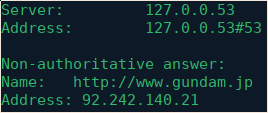
\includegraphics[scale=0.65]{Q1.png}
\caption{}
\end{figure}

According to figure 1, I used the server http://www.gundam.jp, the IP address is 92.242.140.21 \\

\section{Run nslookup to determine the authoritative DNS servers for a university in
Europe.}

\begin{figure}[h!]
\centering
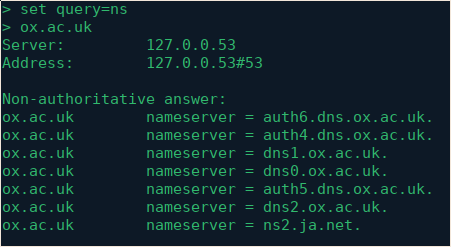
\includegraphics[scale=0.65]{Q2.png}
\caption{}
\end{figure}

According to figure 2, the authoritative DNS server for ox.ac.uk is auth6.dns.ox.ac.uk.\\

\clearpage

\section{Run nslookup so that one of the DNS servers obtained in Question 2 is queried for
the mail servers for Yahoo! mail. What is its IP address?}

\begin{figure}[h!]
\centering
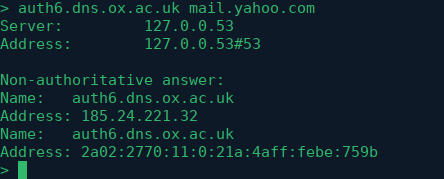
\includegraphics[scale=0.65]{Q3.png}
\caption{}
\end{figure}

According to figure 3, the IP address is 185.24.221.32\\

\begin{figure}[h!]
\centering
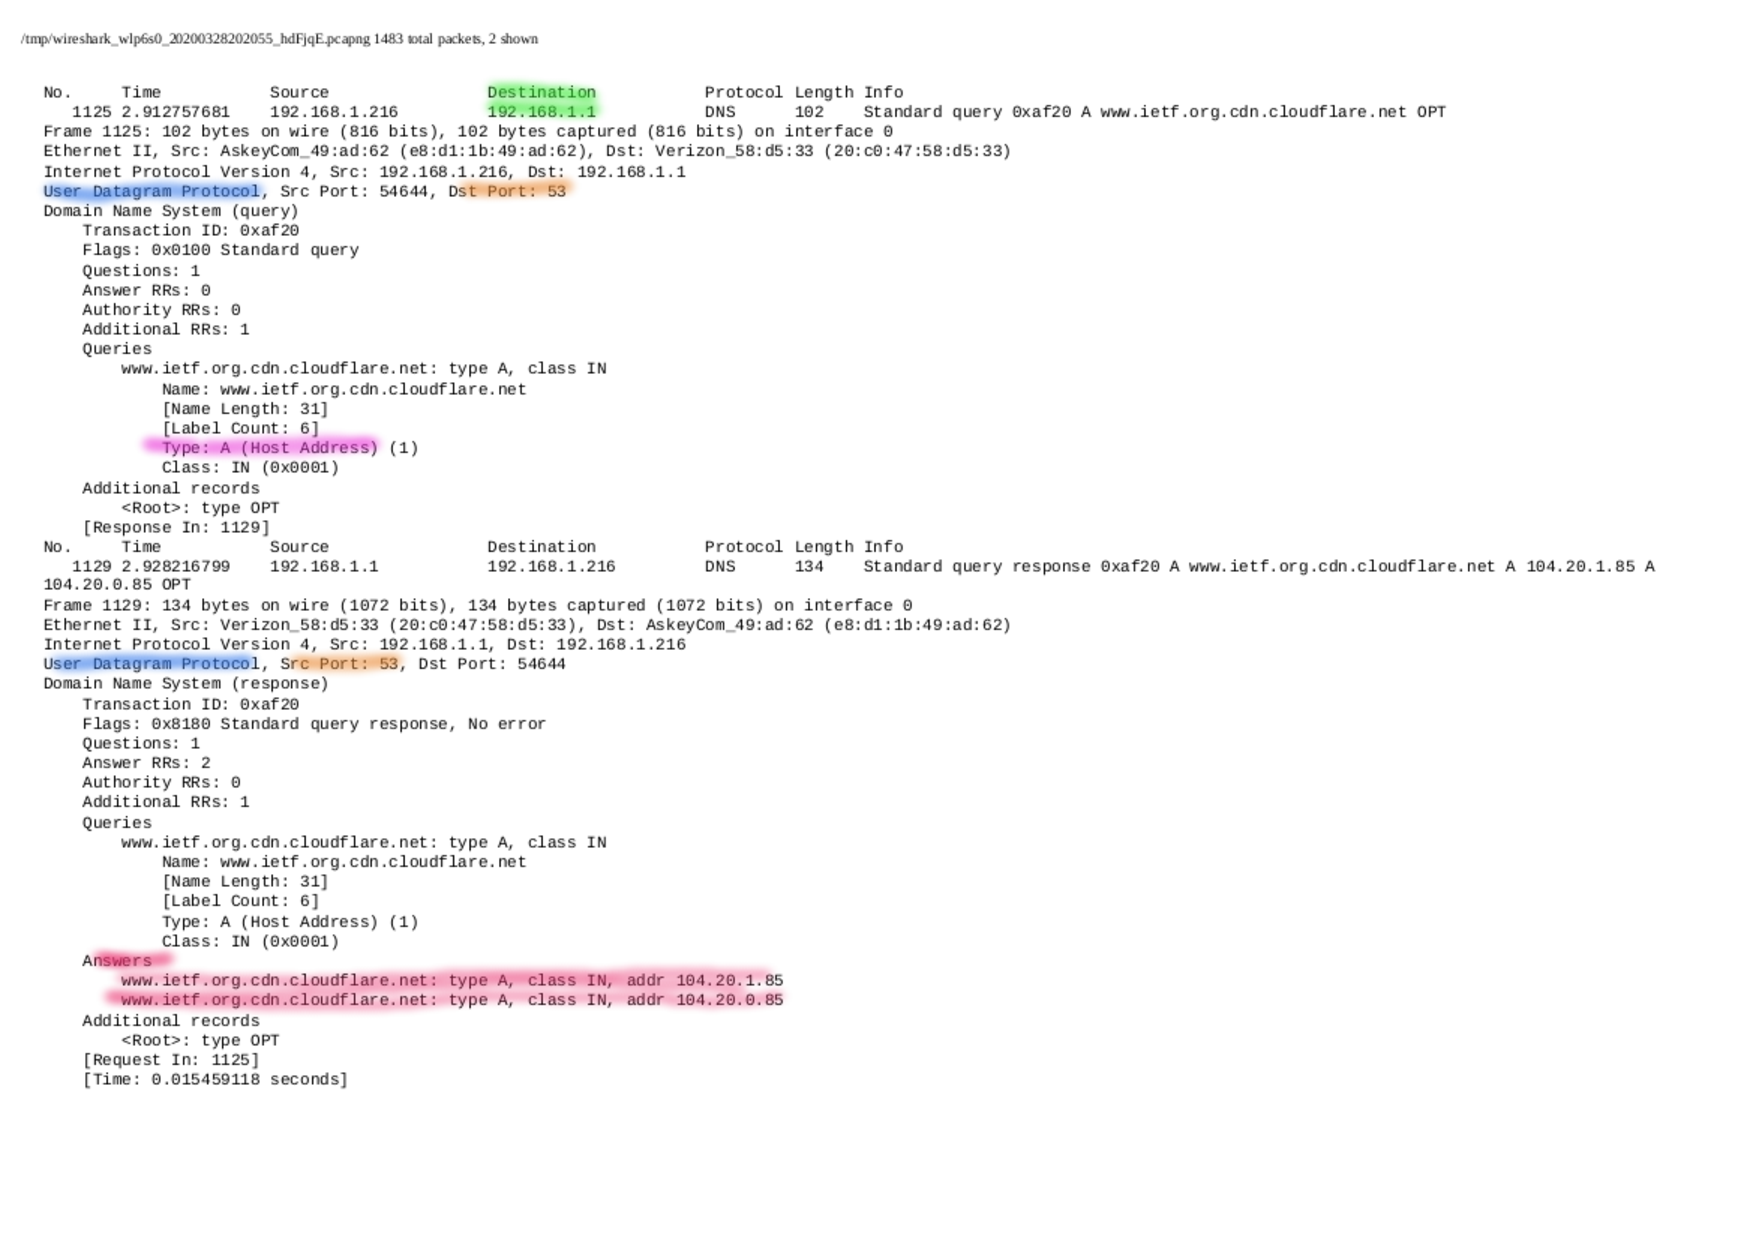
\includegraphics[scale=0.7]{Q4-8.pdf}
\caption{}
\end{figure}

\clearpage

\begin{figure}[h!]
\centering
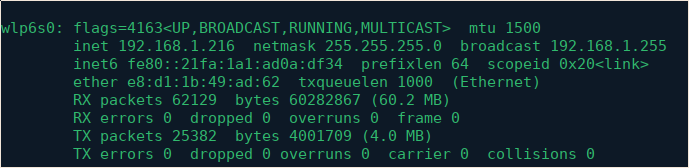
\includegraphics[scale=0.7]{ifconfig.png}
\caption{}
\end{figure}

\section{Locate the DNS query and response messages. Are they sent over UDP or TCP?}
According to figure 4, the query and response messages are sent over UDP.\\

\section{What is the destination port for the DNS query message? What is the source port
of DNS response message?}
According to figure 4, the destination port is 53 and the source port of the response message is also 53.\\

\section{To what IP address is the DNS query message sent? Use ipconfig to determine the
IP address of your local DNS server. Are these two IP addresses the same?}
According to figure 4, the DNS query message is being sent to 192.168.1.1.  According to figure 5, my IP address is 192.168.1.216, thus they are not the same.\\

\section{Examine the DNS query message. What “Type” of DNS query is it? Does the
query message contain any “answers”?}
According to figure 4, it is of type A.  It does not contain answers.\\

\section{Examine the DNS response message. How many “answers” are provided? What
do each of these answers contain?}
According to figure 4, there are 2 answers provided.  The answers contain the address of the website which was queried for.\\

\section{Consider the subsequent TCP SYN packet sent by your host. Does the destination
IP address of the SYN packet correspond to any of the IP addresses provided in
the DNS response message?}
According to figure 6, the IP address of the SYN packed corresponds to the IP address listed in the DNS response message (132.151.6.75).\\

\clearpage

\begin{figure}[h!]
\centering
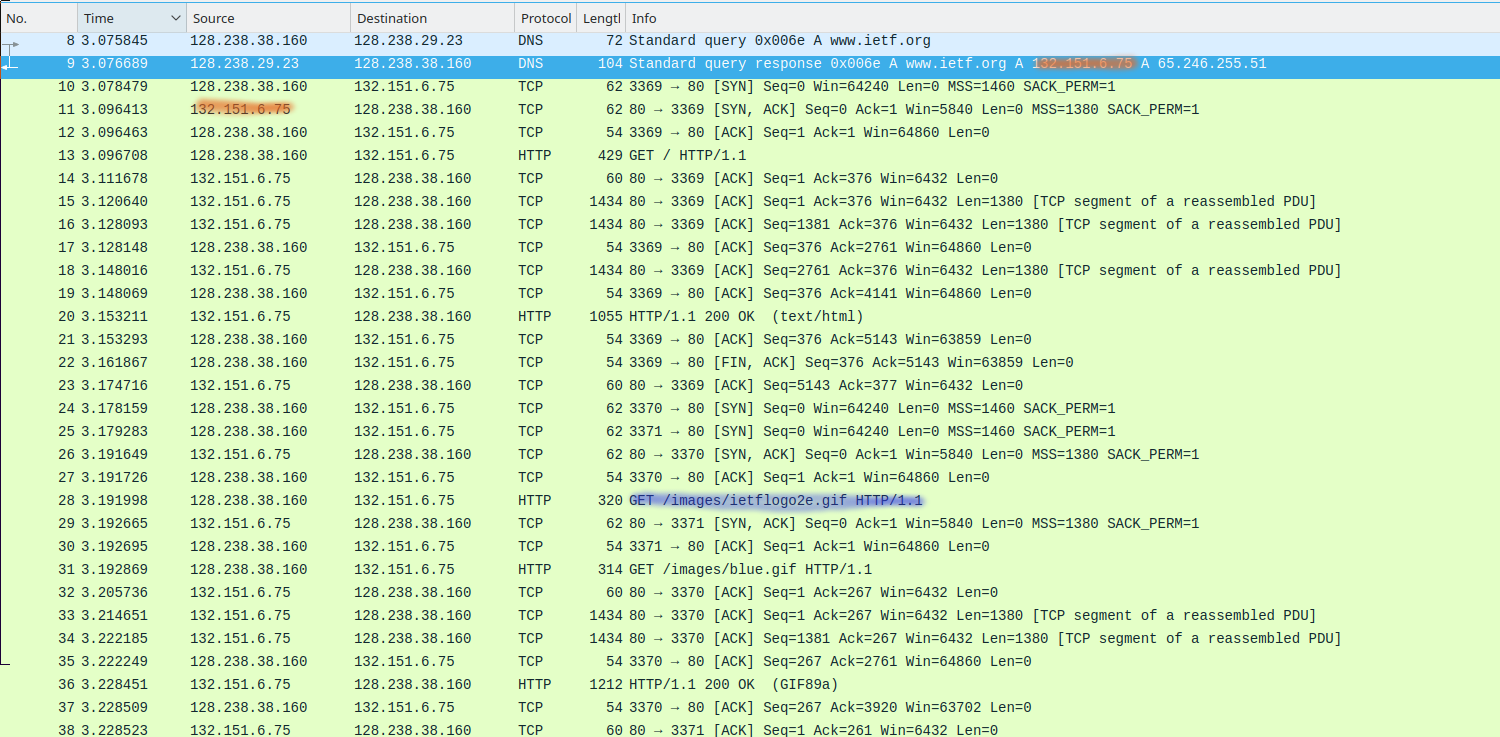
\includegraphics[scale=0.5]{Q9-10.png}
\caption{}
\end{figure}

\section{This web page contains images. Before retrieving each image, does your host
issue new DNS queries?}
According to figure 6, my host does issue new DNS queries after each get request.\\

\clearpage

\begin{figure}[h!]
\centering
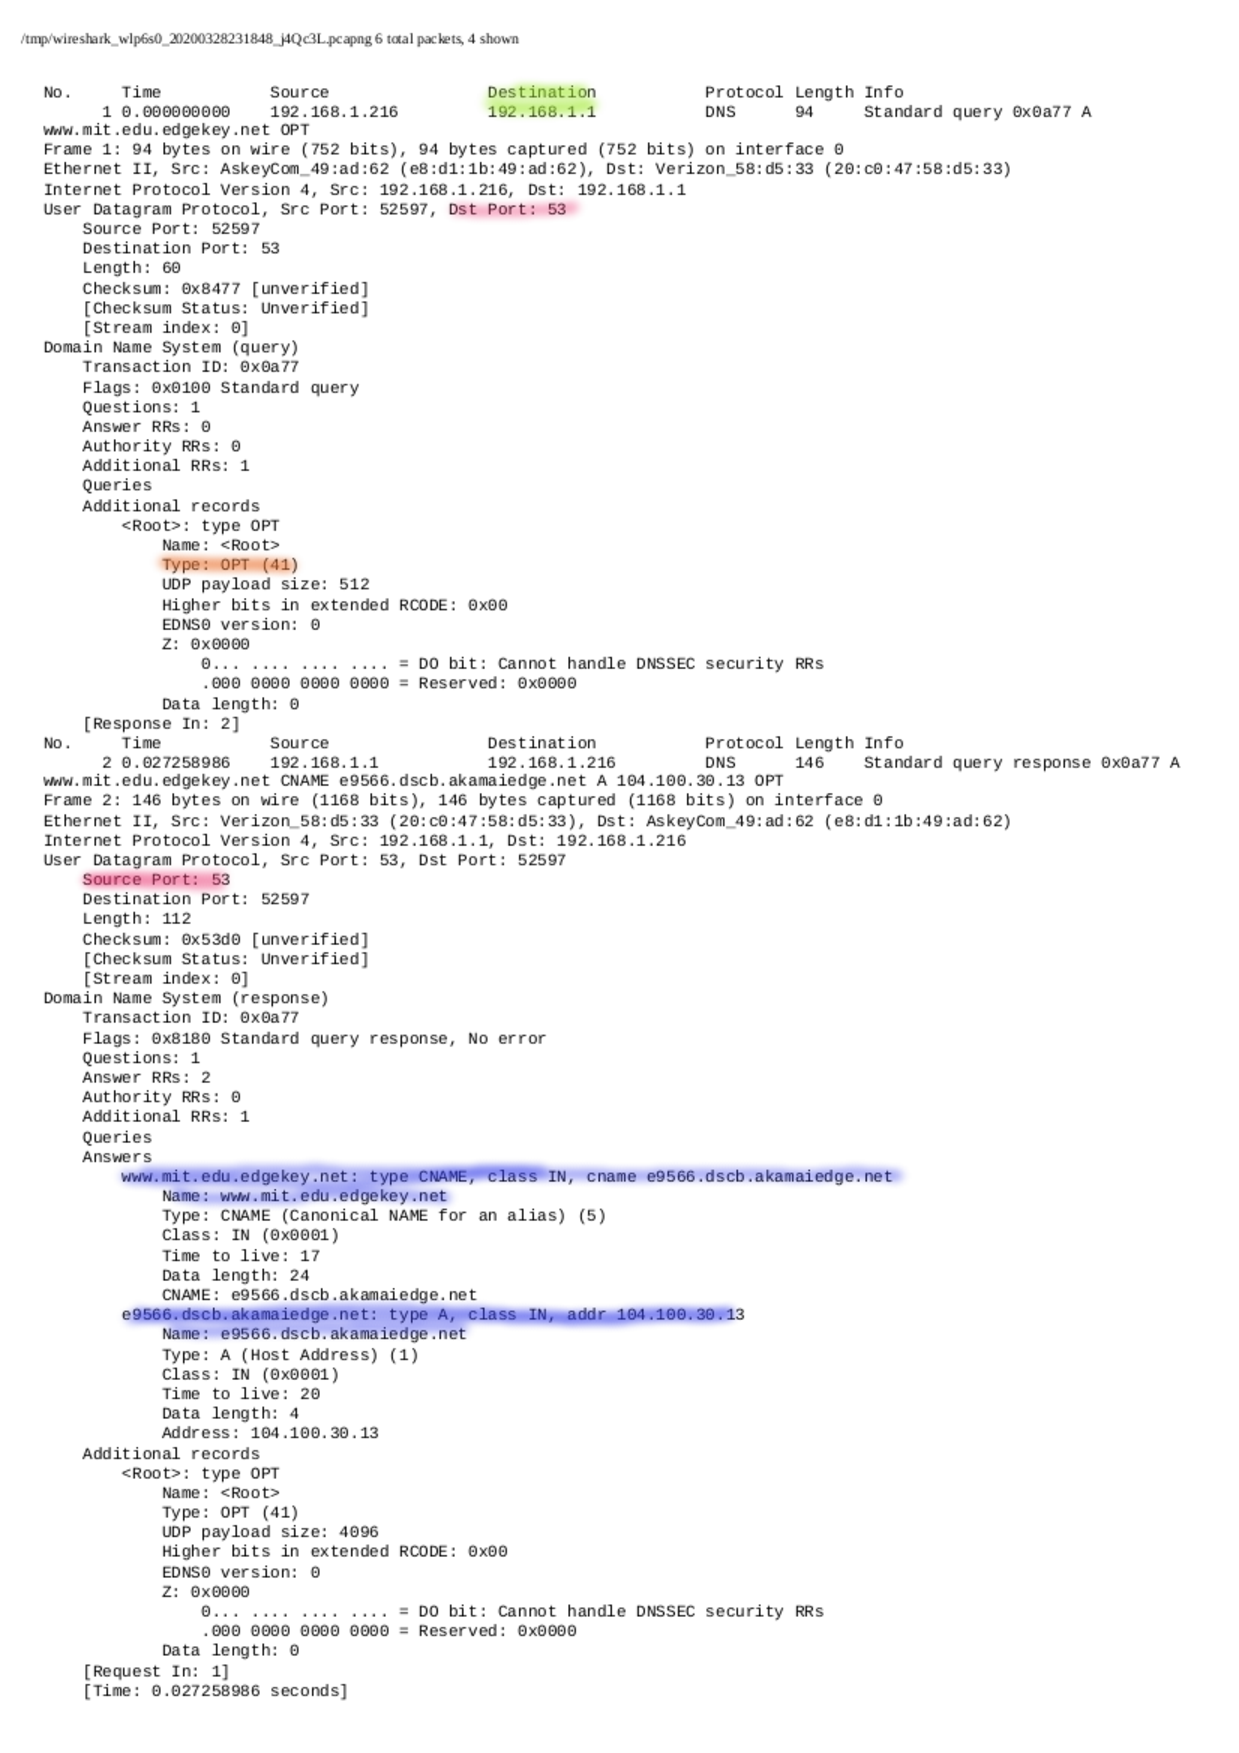
\includegraphics[scale=0.5]{Q11-15.pdf}
\caption{}
\end{figure}

\section{What is the destination port for the DNS query message? What is the source port
of DNS response message?}
According to figure 7, the destination port for the DNS query message is 53, and the source port for the DNS response message is also 53.\\

\section{To what IP address is the DNS query message sent? Is this the IP address of your
default local DNS server?}
According to figure 7, the DNS query message is being sent to 192.168.1.1.  This is not my IP address, as shown in figure 6, my IP is 192.168.1.216.\\

\section{Examine the DNS query message. What “Type” of DNS query is it? Does the
query message contain any “answers”?}
According to figure 7, the query message is of type OPT.  It contains no answers.\\

\section{Examine the DNS response message. How many “answers” are provided? What
do each of these answers contain?}
According to figure 7, there are two answers.  The answers contain a canonical name for an alias, as well as the host address.  The answers also contain the name, type, class, time to live, data length and address.\\

\section{Provide a screenshot}
See figure 7.\\

\begin{figure}[h!]
\centering
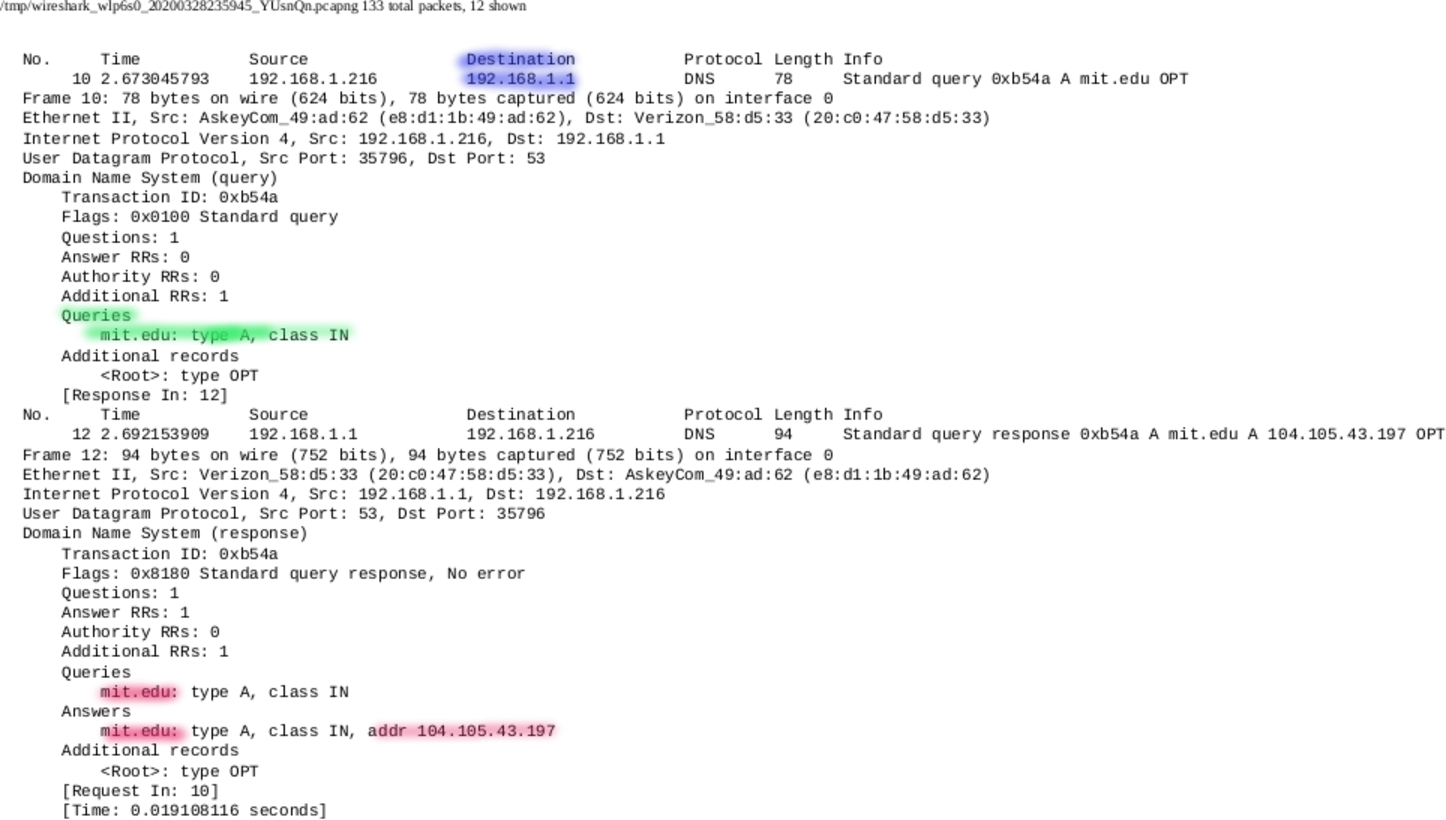
\includegraphics[scale=0.7]{Q16-19.pdf}
\caption{}
\end{figure}


\section{To what IP address is the DNS query message sent? Is this the IP address of your
default local DNS server?}
According to figure 8, the DNS query message is being sent to 192.168.1.1.  This is not the IP of my local default DNS server.\\

\section{Examine the DNS query message. What “Type” of DNS query is it? Does the
query message contain any “answers”?}
According to figure 8, the query is type A.  It doesn't contain any answers.\\

\section{Examine the DNS response message. What MIT nameservers does the response
message provide? Does this response message also provide the IP addresses of the
MIT namesers?}
According to figure 8, the response message provides mit.edu, as well as an IP address of 104.105.43.197.\\

\section{Provide a screenshot.}
See figure 8.\\

\begin{figure}[h!]
\centering
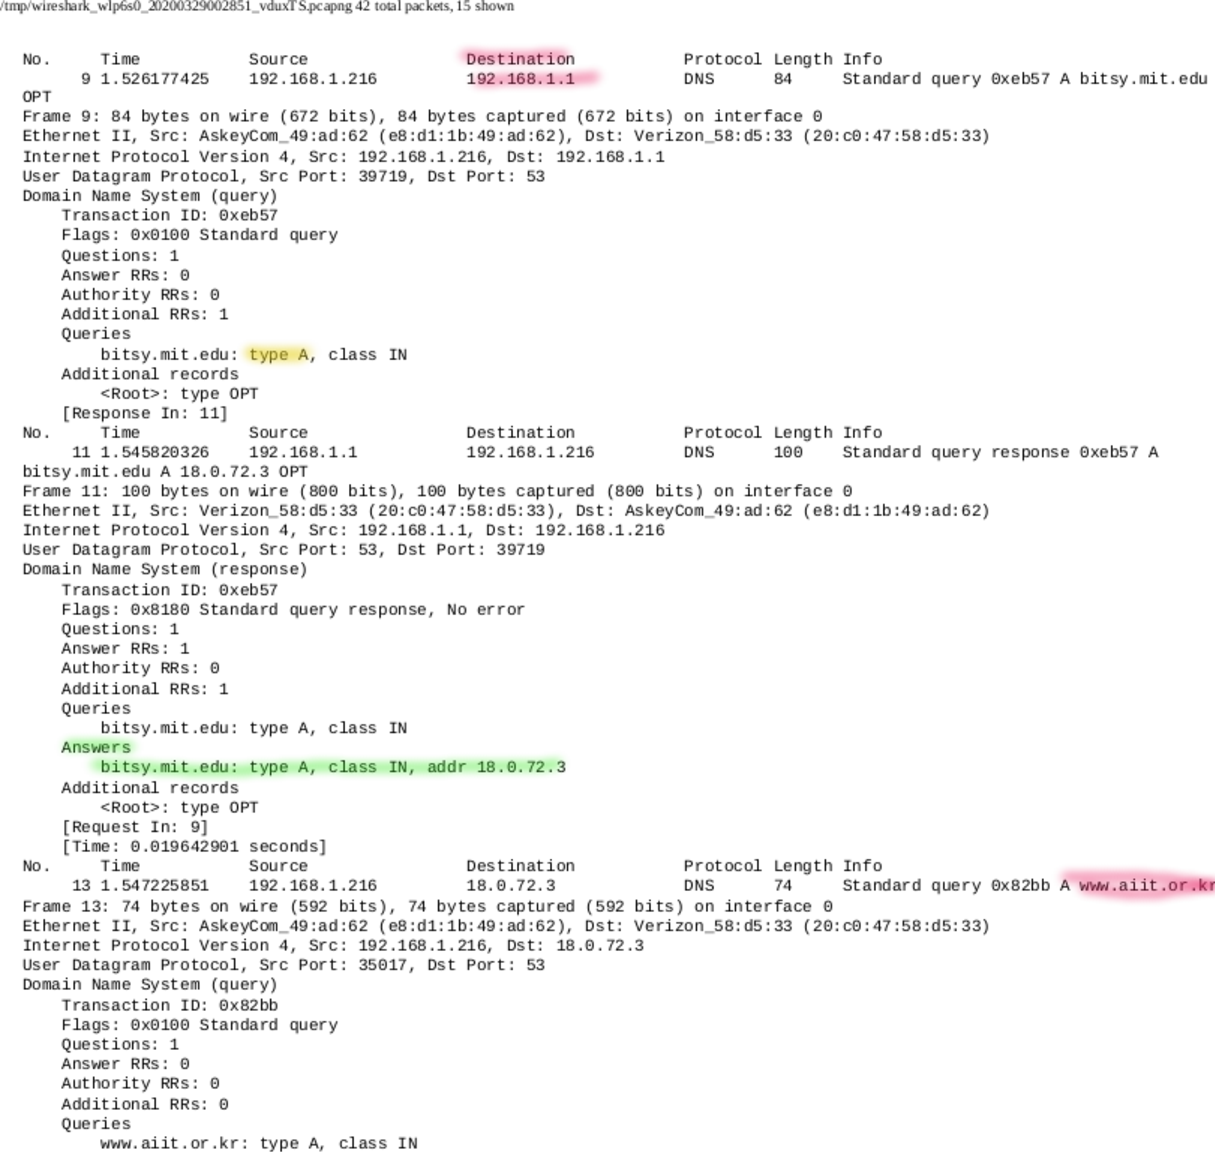
\includegraphics[scale=0.6]{Q20-23.pdf}
\caption{}
\end{figure}

\section{To what IP address is the DNS query message sent? Is this the IP address of your
default local DNS server? If not, what does the IP address correspond to?}
According to figure 9, the DNS query message is being sent to 192.168.1.1, this is not the IP address of my defauly local DNS server.  This IP address corresponds to www.aiit.or.kr

\section{Examine the DNS query message. What “Type” of DNS query is it? Does the
query message contain any “answers”?}
According to figure 9, it is of type A.  It contains no answers.\\

\section{Examine the DNS response message. How many “answers” are provided? What
does each of these answers contain?}
According to figure 9 there is one answer which contains the IP address 18.0.72.3.\\

\section{Provide a screenshot}
See figure 9.\\

\end{document}